\documentclass{standalone}
\usepackage{tikz}

\begin{document}

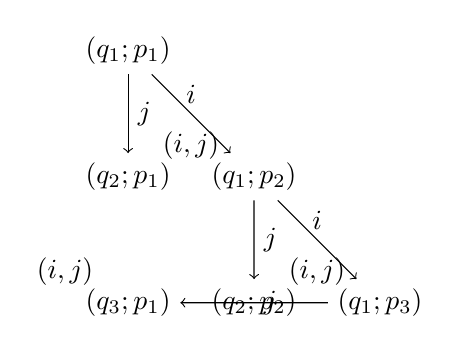
\begin{tikzpicture}[scale=0.8]
    % Define the nodes
    \node (q1p1) at (0,0) {$(q_1; p_1)$};
    \node (q1p2) at (2,-2) {$(q_1; p_2)$};
    \node (q1p3) at (4,-4) {$(q_1; p_3)$};
    \node (q2p1) at (0,-2) {$(q_2; p_1)$};
    \node (q2p2) at (2,-4) {$(q_2; p_2)$};
    \node (q3p1) at (0,-4) {$(q_3; p_1)$};

    % Draw the arrows
    \draw[->] (q1p1) -- node[midway, above] {$i$} (q1p2);
    \draw[->] (q1p2) -- node[midway, above] {$i$} (q1p3);
    \draw[->] (q1p1) -- node[midway, right] {$j$} (q2p1);
    \draw[->] (q1p2) -- node[midway, right] {$j$} (q2p2);
    \draw[->] (q1p3) -- node[midway, right] {$j$} (q3p1);

    % Add labels for clarity
    \node at (1,-1.5) {$(i,j)$};
    \node at (3,-3.5) {$(i,j)$};
    \node at (-1,-3.5) {$(i,j)$};
\end{tikzpicture}

\end{document}